% !TEX TS-program = pdflatexmk

\documentclass[14pt]{beamer}
\usepackage{newtxtext,newtxmath}
\usepackage{microtype}
\usepackage[english]{babel}
\usepackage{hyperref}
\usepackage{graphicx}
\usepackage{listings}
\lstloadlanguages{Python}
\lstset{language=Python}
\lstset{%
basicstyle=\ttfamily\bfseries,
keywordstyle=\color{blue}, emph={self}, emphstyle={\color{blue}},
identifierstyle=,
commentstyle=\color{brown},
stringstyle=\color{green!50!black},
showstringspaces=false,
emphstyle={[2]\color{purple}},
}
\usepackage{tikz}
\usepackage{pgfplots}
\usepackage{forest}
\usetikzlibrary{calc}
\usetikzlibrary{shapes}
\usetikzlibrary{positioning}
\usetikzlibrary{arrows}
\usepackage{array}
\newcolumntype{L}[1]{>{\raggedright\let\newline\\\arraybackslash\hspace{0pt}}m{#1}}

\mode<presentation>{
\usetheme{Madrid}
\definecolor{uabgreen}{cmyk}{.89,.31,.78,.17}
\usecolortheme[named=uabgreen]{structure}
\setbeamertemplate{navigation symbols}{}
\setbeamertemplate{footline}[frame number]
\setbeamertemplate{section in toc}[square]
\setbeamertemplate{subsection in toc}[square]
\setbeamertemplate{items}[square]
\setbeamercovered{transparent=5}
}

\newcommand{\keyword}[1]{{\color{blue}#1}}
\newcommand{\cmnt}[1]{{\color{gray}#1}}
\newcommand{\str}[1]{{\color{green!50!black}#1}}
\newcommand{\num}[1]{{\color{green!55!blue}#1}}
\newcommand{\defn}[1]{{\color{purple}#1}}

\newcommand{\limpl}{\Rightarrow}
\newcommand{\liff}{\Leftrightarrow}

\newcommand{\tab}{\hspace{1em}}

\author[Dr. Bethard]{Dr. Steven Bethard}
\institute[UAB CIS]{%
Computer and Information Sciences\\
University of Alabama at Birmingham}

\AtBeginSection[]
{
  \begin{frame}<beamer>{Outline}
    \tableofcontents[currentsection]
  \end{frame}
}

\tikzset{
  invisible/.style={opacity=0,text opacity=0},
  text visible on/.code={%
    \alt<#1>{}{\pgfkeysalso{text opacity=0}}
  },
  visible on/.code={%
    \alt<#1>{}{\pgfkeysalso{invisible}}
  },
  filled on/.code={%
    \alt<#1>{\pgfkeysalso{fill=gray}}{}
  },
  alt/.code n args={3}{%
    \alt<#1>{\pgfkeysalso{#2}}{\pgfkeysalso{#3}}
  },
}
\forestset{
  edge weight/.style={
    edge label={node[midway,above,sloped]{#1}}},
  invisible/.style={
    /tikz/invisible,
    edge={/tikz/invisible}},
  visible on filled on/.code n args={2}{%
    \alt<#1>{\alt<#2>{\pgfkeysalso{fill=gray}}{}}{\pgfkeysalso{invisible}}
  },
  visible on/.code={%
    \alt<#1>{}{\pgfkeysalso{invisible}}
  },
}

\newlength{\wumpusgridsize}
\newenvironment{wumpusgrid}[2]{%
\setlength{\wumpusgridsize}{#2}
\begin{tikzpicture}
\draw[very thick,step=\wumpusgridsize] (0,0) grid (#1\wumpusgridsize, #1\wumpusgridsize);
}{%
\end{tikzpicture}
}
\newcommand{\wumpustop}[5][]{%
\only<#2>{\node[#1] at (#3\wumpusgridsize+0.5\wumpusgridsize,#4\wumpusgridsize+0.75\wumpusgridsize) {#5};}
}
\newcommand{\wumpusbottom}[5][]{%
\only<#2>{\node[#1] at (#3\wumpusgridsize+0.5\wumpusgridsize,#4\wumpusgridsize+0.25\wumpusgridsize) {#5};}
}
\newcommand{\wumpusagent}[3]{\wumpusbottom{#1}{#2}{#3}{\fbox{A}}}
\newcommand{\wumpuspercept}[4]{%
\only<#1>{\node[red,inner sep=0pt] at (#2\wumpusgridsize+0.25\wumpusgridsize,#3\wumpusgridsize+0.75\wumpusgridsize) {\textbf{#4}};}
}
\newcommand{\wumpusknowledge}[4]{%
\only<#1>{\node[draw,cloud,inner sep=0pt,text width=1em,align=center] at (#2\wumpusgridsize+0.75\wumpusgridsize,#3\wumpusgridsize+0.75\wumpusgridsize) {\footnotesize #4};}
}

\lstset{emph={[2]__init__,__str__}}

\title{Constraint Satisfaction Problems}
\date[]{6 Feb 2014}

\newcommand{\V}[1]{\mbox{\texttt{#1}}}
\newcommand{\VeqV}[2]{$\V{#1} = \V{#2}$}
\newcommand{\VneqV}[2]{$\V{#1} \neq \V{#2}$}
\newcommand{\assignment}[1]{%
$
\left\{
\mbox{#1}
\right\}
$}

\begin{document}

\begin{frame}
  \titlepage
\end{frame}

\begin{frame}{Outline}
  \tableofcontents
\end{frame}

\section{Constraint Satisfaction}

\subsection{Defining Problems}
\begin{frame}{Example: Map Coloring}
	\begin{columns}
		\begin{column}{1.5in}
			\begin{block}{Problem}
				Color all countries with red, green or blue,
				and with no 2 adjacent countries the same color
			\end{block}
		\end{column}
		\begin{column}{2.5in}
			\only<1>{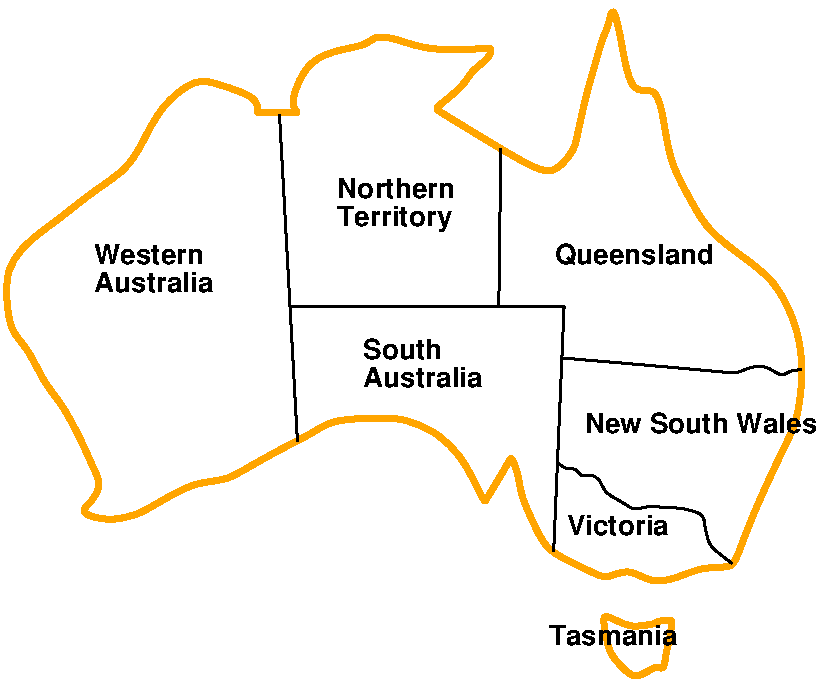
\includegraphics[height=1.75in]{australia.pdf}}%
			\only<2->{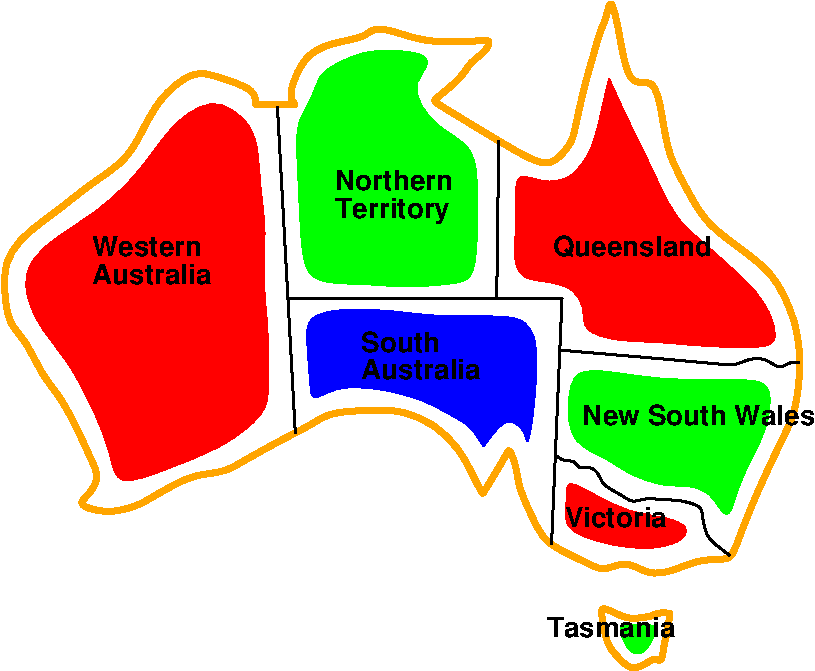
\includegraphics[height=1.75in]{australia-solution.pdf}}%
		\end{column}
	\end{columns}
\end{frame}
\begin{frame}{Constraint Satisfaction Problem Definition}
	\begin{block}{Terms}
		\begin{description}[Constraints]
			\item[Variables] $X_1, X_2, \ldots, X_n$
			\item[Domains] Allowable values for each variable
			\item[Constraints] Allowable combinations of variables
		\end{description}
	\end{block}
	\begin{block}{States}
		\begin{description}
			\item[Assignment] of values to variables, $\{X_i=v_i, X_j=v_j, \ldots\}$
		\end{description}
	\end{block}
	\begin{block}{Types of States}
		\begin{description}[Consistent]
			\item[Consistent] No constraints violated
			\item[Solution] No constraints violated, all variables assigned
		\end{description}
	\end{block}
\end{frame}
\begin{frame}{Example: Map Coloring}
	\begin{columns}
		\begin{column}{1.5in}
			\begin{block}{Problem}
				Color all countries with red, green or blue,
				and with no 2 adjacent countries the same color
			\end{block}
		\end{column}
		\begin{column}{2.5in}
			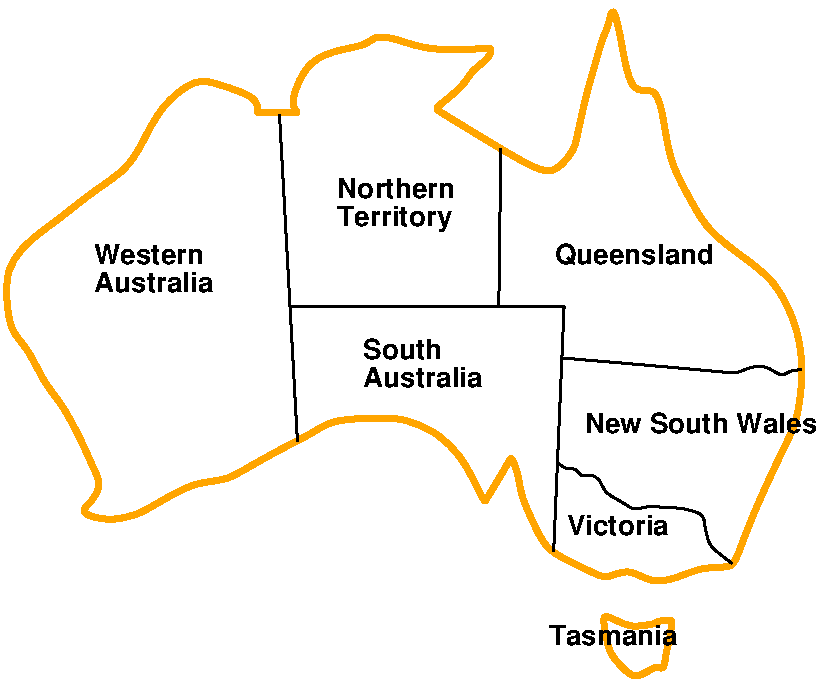
\includegraphics[height=1.75in]{australia.pdf}
		\end{column}
	\end{columns}
	\begin{description}[Constraints]
		\item[Variables] \uncover<2->{\V{WA}, \V{NT}, \V{Q}, \V{NSW}, \V{V}, \V{SA}, \V{T}}
		\item[Domains] \uncover<3->{$D_i = \{\V{red}, \V{green}, \V{blue}\}$}
		\item[Constraints] \uncover<4->{\VneqV{WA}{NT}, \VneqV{WA}{SA}, \VneqV{NT}{SA}, \ldots}
		\item[Solution] \uncover<5->{\assignment{%
			\begin{tabular}{l}
			\VeqV{WA}{red}, \VeqV{NT}{green}, \VeqV{Q}{red}, \\
			\VeqV{NSW}{green}, \VeqV{V}{red}, \VeqV{SA}{blue}, \\
			\VeqV{T}{green}
			\end{tabular}}}
	\end{description}
\end{frame}
\begin{frame}{Example: Cryptarithmetic}
\begin{center}
\large
$
\begin{array}{ c c c c }
& T & W & O \\
+ & T & W & O \\
\hline
F & O & U & R
\end{array}
$
\end{center}
	\begin{description}[Constraints]
		\item[Variables] \uncover<2->{$T, W, O, F, U, R\uncover<5->{, C_1, C_2, C_3$}}
		\item[Domains] \uncover<3->{$\{0, 1, 2, 3, 4, 5, 6, 7, 8, 9\}$}
		\item[Constraints] \uncover<4->{$
			\begin{array}[t]{lll}
			O + O       & = & R + 10 \cdot C_1 \\
			C_1 + W + W & = & U + 10 \cdot C_2 \\
			C_2 + T + T & = & O + 10 \cdot C_3 \\
			C_3         & = & F
			\end{array}
			$}
		\item[Solution] \uncover<6->{$\left\{\begin{array}{l}T=7, W=3, O=4, F=1, U=6,\\R=8, C_1=0, C_2=0, C_3=1\end{array}\right\}$}
	\end{description}
\end{frame}
\begin{frame}{Example: Meeting Scheduling}
	\begin{block}{Problem Description}
		\begin{itemize}
			\item 2 hour meetings: Jim \& Tammy
			\item 1 hour meetings: Jim \& Martha, Martha \& Tammy
			\item 9:00am and 5:00pm, 1 hour between meetings
			\item Busy: Jim 12-2, Martha 11-1, Tammy 10-11 and 2-3
		\end{itemize}
	\end{block}
	\begin{description}[Constraints]
		\item[Variables] \visible<2->{\V{J\&T}, \V{J\&M}, \V{M\&T}}
		\item[Domains] \visible<2->{
			$D_{\V{\scriptsize J\&T}} = \{\V{9-11}, \V{10-12}, \ldots\}$ \\
			$D_{\V{\scriptsize J\&M}} = D_{\V{\scriptsize M\&T}} = \{\V{9-10}, \V{10-11}, \ldots\}$}
		\item[Constraints] \visible<2->{
			$\V{J\&T} \cap \V{J\&M} = \emptyset$, $\V{J\&M} \cap \V{M\&T} = \emptyset$, \\
			$\V{12-2} \cap \V{J\&T} = \emptyset$, $\V{12-2} \cap \V{J\&M} = \emptyset$, \ldots}
		\item[Solution] \visible<2->{
			$\{\V{J\&T}=\V{3-5}, \V{M\&T}=\V{1-2}, \V{J\&M}=\V{10-11}\}$}
	\end{description}
\end{frame}

\subsection{Problem Types}
\begin{frame}{Domain Types}
	\begin{block}{Finite Domains}
		\begin{itemize}
			\item Examples: map coloring, 8-queens
			\item Constraints described by enumeration, e.g. \\
			      $(\V{WA}, \V{NT}) \in \{(\V{red}, \V{green}), (\V{red}, \V{blue}), \ldots\}$
		\end{itemize}
	\end{block}
	\pause
	\begin{block}{Infinite but Countable Domains}
		\begin{itemize}
			\item Examples: scheduling jobs by day or hour
			\item Need constraint language, e.g.
			      \small $\V{Start}_{\V{\scriptsize Job1}} + 5 \leq \V{Start}_{\V{\scriptsize Job3}}$
		\end{itemize}
	\end{block}
	\pause
	\begin{block}{Continuous Domains}
		\begin{itemize}
			\item Examples: scheduling jobs by any fraction of time
			\item Some can be solved by linear programming
		\end{itemize}
	\end{block}
\end{frame}
\begin{frame}{Constraint Types}
	\begin{block}{Unary Constraints}
		\begin{itemize}
			\item Restrict the value of a single variable
			\item<2-> Can be eliminated by preprocessing domains
		\end{itemize}
	\end{block}
	\begin{block}<3->{Binary Constraints}
		\begin{itemize}
			\item Relate two variables, e.g. $\V{SA} \neq \V{NSW}$
		\end{itemize}
	\end{block}
	\pause
	\begin{block}<4->{Higher Order Constraints}
		\begin{itemize}
			\item Relate more than two variables\uncover<5->{: can convert to binary}
		\end{itemize}
	\end{block}
	\begin{block}<6->{Preferences}
		\begin{itemize}
			\item Cost of assignments, e.g. \V{red} is better than \V{green}
		\end{itemize}
	\end{block}
\end{frame}


\section{Backtracking Search}

\subsection{CSPs as Search}
\begin{frame}{CSPs as Search}
	\begin{block}{Formulation}
		\begin{description}[Actions]
			\item[States] Full or partial assignments
			\item[Initial] The empty assignment, $\{\}$
			\item[Actions] Assign value to variable, obeying constraints
			\item[Goal] Assignment is complete
		\end{description}
	\end{block}
	\begin{block}<2->{Benefits}
		\begin{itemize}
			\item Same for all CSPs
			\item All solutions at depth $n$ 
			      \uncover<3->{$\Rightarrow$ depth-first search ok}
		\end{itemize}
	\end{block}
\end{frame}
\begin{frame}{CSPs as Search}
	\begin{block}{Problem}
		Given $n$ variables, $d$ values in domains:
		\\ \smallskip
		\begin{tabular}{|lllll|}
			\hline
			                     & \color{blue}Root & \color{blue}Level 1 & \color{blue} Level 2 & \color{blue}\ldots \\
			\color{blue}Branches & \pause $nd$      & \pause $(n - 1)d$   & \pause $(n - 2)d$    & \ldots \\
			\hline
		\end{tabular}
		\\ \smallskip
		\pause Leaves: \pause $n! \cdot d^n$ \pause \hspace{2em} Total possible assignments: \pause \alert{$d^n$}
	\end{block}
	\pause
	\begin{block}{Note}
		Variable assignments are commutative, e.g.
		\begin{itemize}
			\item $\V{WA}=\V{red}$ then $\V{NT}=\V{green}$
			\item $\V{NT}=\V{green}$ then $\V{WA}=\V{red}$
		\end{itemize}
	\end{block}
	\pause
	{\color{blue}Solution}: Consider only one variable at each node
\end{frame}
\begin{frame}[fragile]{Backtracking Search Code}
	\scriptsize
	\begin{semiverbatim}\bfseries
		\keyword{def} \defn{csp_search}(csp, heuristic, assignment=\keyword{None}):
		    \pause\keyword{if} assignment \keyword{is} \keyword{None}:
		        assignment = \{\}
		    \pause\cmnt{# if assignment is complete, return it}
		    \keyword{if} len(assignment) == len(csp.variables):
		        \keyword{return} assignment
		    \pause\cmnt{# select an unassigned variable and order the values}
		    variable = heuristic.select_variable(csp, assignment)
		    \pause\cmnt{# try assigning each value to the variable}
		    \keyword{for} value \keyword{in} heuristic.order_values(csp, assignment, variable):
		        assignment[variable] = value
		        \pause\cmnt{# for consistent assignments, recursively check if
		        # it is possible to assign the remaining variables}
		        \keyword{if} csp.is_consistent(assignment):
		            result = csp_search(csp, heuristic, assignment)
		            \keyword{if} result \keyword{is} \keyword{not} \keyword{None}:
		                \keyword{return} result
		        \pause\keyword{del} assignment[variable]
		    \cmnt{# all assignments failed}
		    \keyword{return} \keyword{None}
	\end{semiverbatim}
\end{frame}
\begin{frame}[label=backtracking-example]{Backtracking Example}
\begin{description}[Constraints]
\item[Variables] \V{WA}, \V{NT}, \V{Q}, \V{SA}, \V{NSW}, \V{V}, \V{T}
\item[Domains] $D_i = \{\V{red}, \V{green}, \V{blue}\}$
\item[Constraints] \VneqV{SA}{WA}, \VneqV{SA}{NT}, \VneqV{SA}{Q}, \VneqV{SA}{NSW}, \VneqV{SA}{V}, \VneqV{WA}{NT}, \VneqV{NT}{Q}, \VneqV{Q}{NSW}, \VneqV{NSW}{V}
\end{description}
\footnotesize
\begin{forest}
[{\assignment{}},visible on={2-}
  [{\assignment{\V{WA}=\V{red}}},visible on={3-}
    [{\assignment{
        \VeqV{WA}{red},
        \VeqV{NT}{green}}},visible on={4-}
      [{\assignment{
          \VeqV{WA}{red},
          \VeqV{NT}{green},
          \VeqV{Q}{blue}}},visible on={5-6}
          [{\assignment{
          \VeqV{WA}{red},
          \VeqV{NT}{green},
          \VeqV{Q}{blue},
          \VeqV{SA}{???}}},visible on={6}]
      ]
      [{\assignment{
          \VeqV{WA}{red},
          \VeqV{NT}{green},
          \VeqV{Q}{red}}},visible on={7-}
          [{\ldots},visible on={8-}]
      ]
    ]
    [{\ldots},invisible]
  ]
  [{\ldots},invisible]
]
\end{forest}
\end{frame}

\subsection{Search Heuristics}
\begin{frame}{Backtracking Heuristics}
	\begin{block}{Problem}
		\begin{itemize}
			\item Basic depth first search is still too inefficient.
			\item E.g. Can only solve $n$-queens for $n \approx 25$
		\end{itemize}
	\end{block}
	\begin{block}{How can we be smarter?}
		\begin{itemize}
			\pause
			\item Which variable should be assigned next?
			\pause
			\item In what order should its values be tried?
			\pause
			\item Can we detect inevitable failure early?
		\end{itemize}
	\end{block}
\end{frame}
\begin{frame}{Minimum Remaining Values}
	\begin{block}{Idea}
		Select the variable with the fewest legal values \\
	\end{block}
	\pause
	\begin{center}
		\visible<2->{
\includegraphics[width=4in]{australia-most-constrained-variable.pdf}}
	\end{center}
	\pause
	\begin{block}{Also Known As}
		Most Constrained Variable
	\end{block}
\end{frame}
\begin{frame}{Degree Heuristic}
	\begin{block}{Idea}
		\begin{itemize}
			\item But what to do when MRV produces ties?
			\item Select variable with most constraints on other values
		\end{itemize}
	\end{block}
	\pause
	\begin{center}
		\visible<2->{
\includegraphics[width=4in]{australia-most-constraining-variable.pdf}}
	\end{center}
	\pause
	\begin{block}{Also Known As}
		Most Constraining Variable
	\end{block}
\end{frame}
\begin{frame}{Least Constraining Value}
	\begin{block}{Idea}
		Select the variable that rules out the smallest
		number of values for the remaining variables
	\end{block}
	\pause
	\begin{center}
		\visible<2->{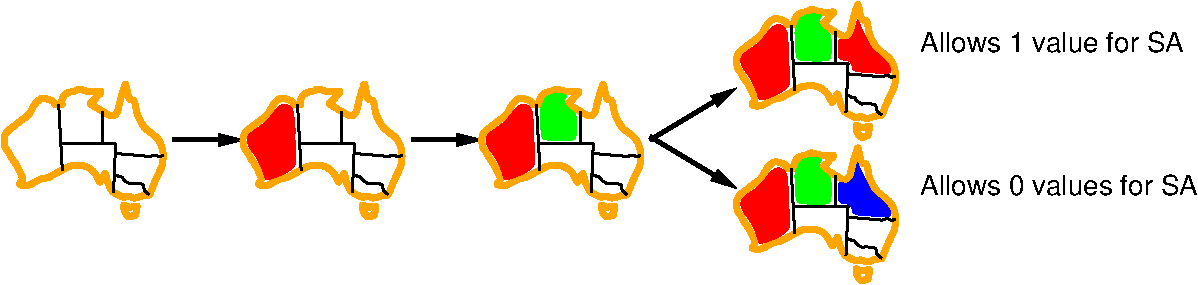
\includegraphics[width=4in]{australia-least-constraining-value.pdf}}
	\end{center}
	\pause
	\begin{tabular}{ll}
		          & Minimum Remaining Values \\
		+         & Degree Heuristic \\
		+         & Least Constraining Value \\
		\hline
		$\approx$ & 1000 queens
	\end{tabular}
\end{frame}
\begin{frame}[t]{Forward Checking}
	\begin{block}{Idea}
		\begin{itemize}
			\item Keep track of remaining legal values for all variables
			\item Stop search when any variable has no legal values
		\end{itemize}
	\end{block}
	\only<1>{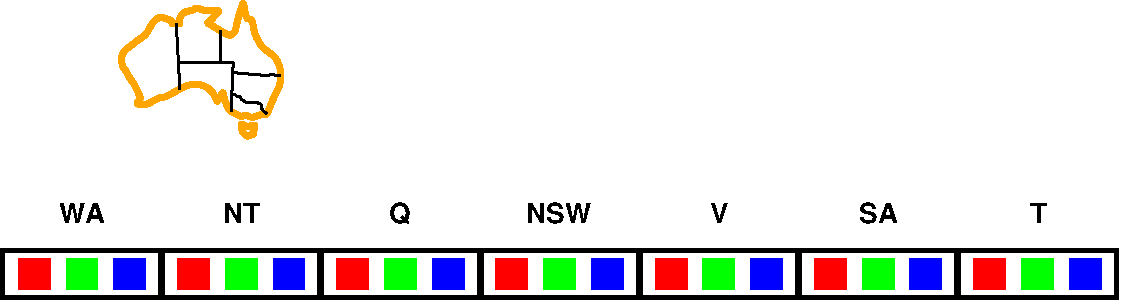
\includegraphics[width=4in]{forward-checking-progress-1.pdf}}%
	\only<2>{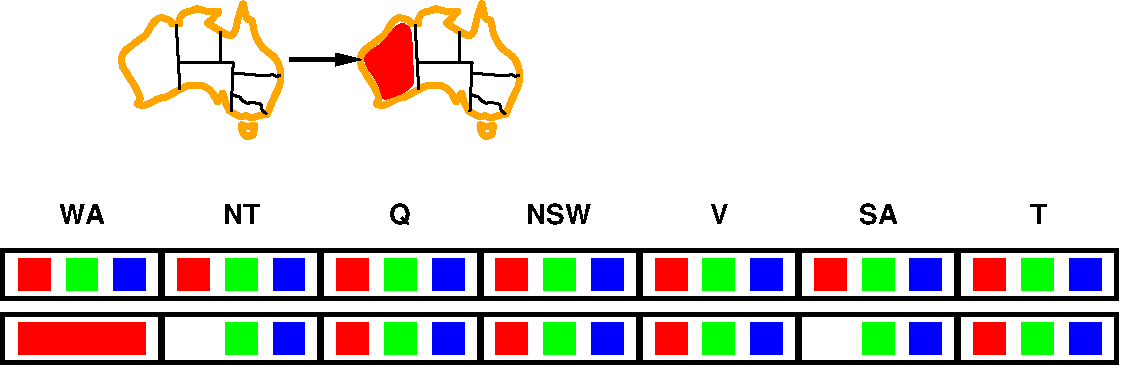
\includegraphics[width=4in]{forward-checking-progress-2.pdf}}%
	\only<3>{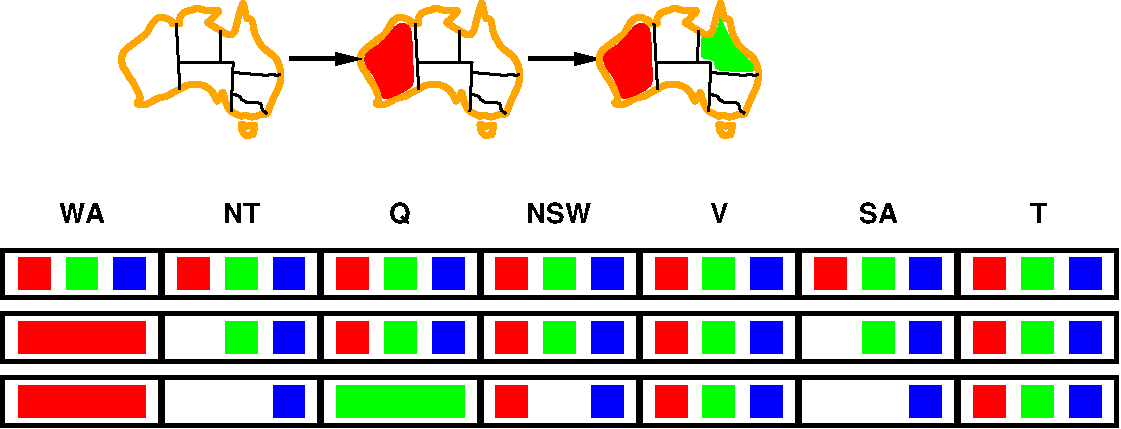
\includegraphics[width=4in]{forward-checking-progress-3.pdf}}%
	\only<4>{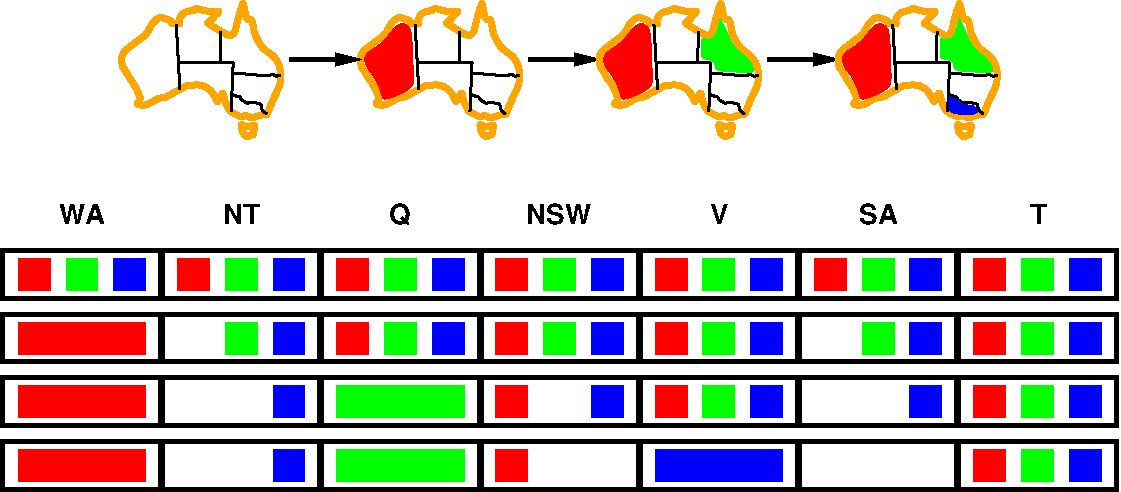
\includegraphics[width=4in]{forward-checking-progress-4.pdf}}%
\end{frame}

\section{Search Alternatives}

\subsection{Local Search}
\begin{frame}{CSPs as Local Search}
	\begin{block}{Formulation}
		\begin{description}
			\item[States] Complete assignments
			\item[Initial] Any complete assignment
			\item[Actions] Change value of one variable
			\item[Goal] Consistent assignment
		\end{description}
	\end{block}
	\pause
	\begin{block}{Benefits}
		\begin{itemize}
			\item Minimal memory consumption
			\item Emprically very effective
		\end{itemize}
	\end{block}
\end{frame}
\begin{frame}{Min-Conflicts}
	\begin{block}{Idea}
		\begin{itemize}
			\item Pick a variable with constraint violations
			\item Assign the value that violates the fewest constraints
		\end{itemize}
	\end{block}
	\begin{center}
		\visible<2>{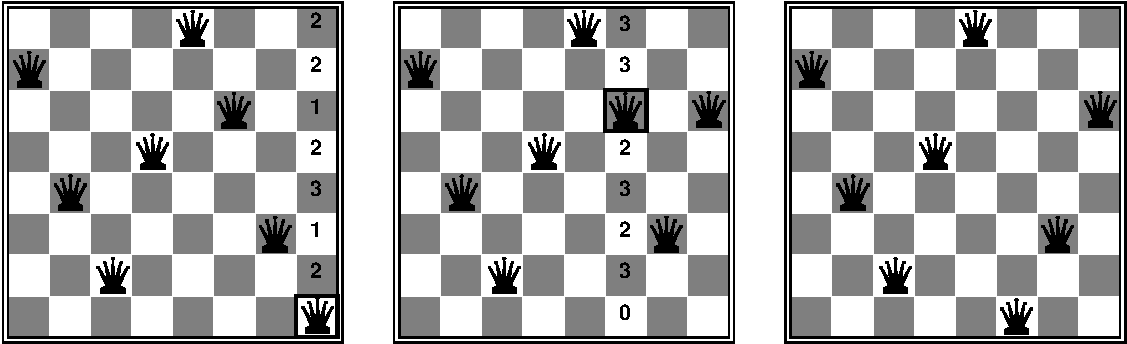
\includegraphics[width=4in]{8-queens-min-conflicts.pdf}}
	\end{center}
\end{frame}
\begin{frame}[fragile]{Min-Conflicts Code}
	\scriptsize
	\begin{semiverbatim}\bfseries
		\keyword{def} \defn{min_conflicts}(csp, max_steps):
		    \pause\cmnt{# start with an initial complete assignment}
		    assignment = \{\}
		    \keyword{for} variable \keyword{in} csp.variables:
		        assignment[variable] = random.choice(variable.domain)
		    \pause\cmnt{# adjust one variable each time through the loop}
		    \keyword{for} i \keyword{in} range(max_steps):
		        \pause\cmnt{# return the assignment when it is consistent}
		        \keyword{if} csp.is_consistent(assignment):
		            \keyword{return} assignment
		        \pause\cmnt{# otherwise, select a random conflicted variable}
		        var = random.choice(csp.get_conflicts(assignment))
		        \pause\cmnt{# assign the variable the value with minimal conflicts}
		        counts = \{\}
		        \keyword{for} value \keyword{in} var.domain:
		            assignment[var] = value
		            counts[value] = len(csp.get_conflicts(assignment))
		        assignment[var] = min(counts, key=counts.get)
		    \pause\cmnt{# all assignments failed}
		    \keyword{return} \keyword{None}
	\end{semiverbatim}
\end{frame}
\begin{frame}{Min-Conflicts Properties}
	\begin{block}{$n$-Queens}
		Almost constant time for arbitrary $n$ with high probability
	\end{block}
	\pause
	\begin{block}{Other kinds of CSPs}
		\begin{columns}
			\begin{column}{1.5in}
				Appears the same is true except for a narrow range of:
				\[
					R = \frac{\left|\mbox{constraints}\right|}{\left|\mbox{variables}\right|}
				\]
			\end{column}
			\begin{column}{2in}
				\begin{center}
					\visible<2>{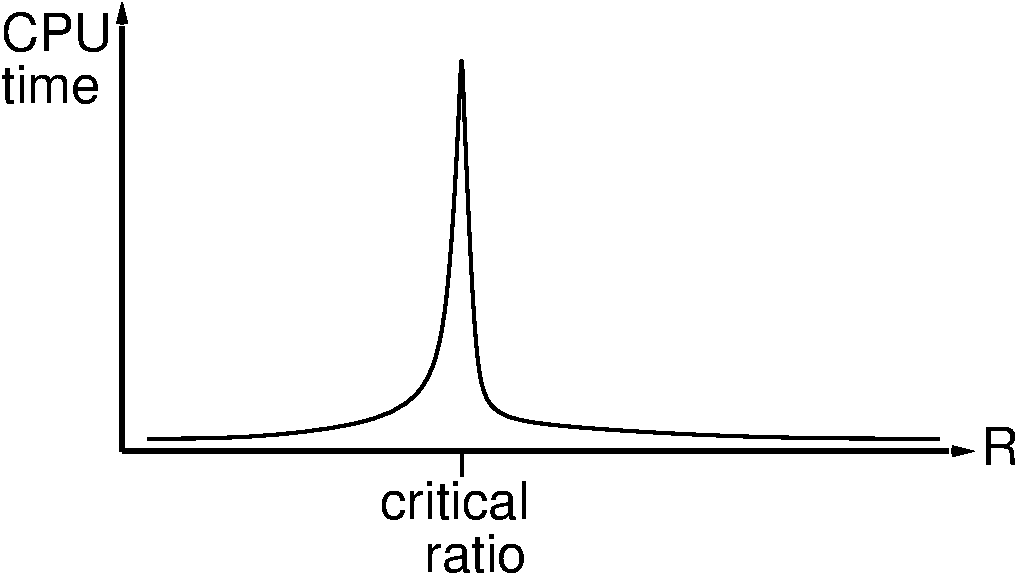
\includegraphics[width=2in]{random-csp-runtime.pdf}}
				\end{center}
			\end{column}
		\end{columns}
	\end{block}
\end{frame}

\subsection{Tree Search}
\begin{frame}[label=tree-csp]{Tree-Structured CSPs}
\begin{columns}[T]
\begin{column}{0.5\textwidth}
CSPs as graphs:
\begin{itemize}
\item Nodes = Variables
\item Edges = Constraints
\end{itemize}
\end{column}
\begin{column}{0.5\textwidth}
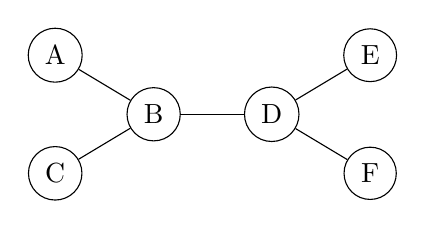
\begin{tikzpicture}[every node/.style={draw,circle}]
\node at (0, 1.5) (A) {A};
\node at (1.25, 0.75) (B) {B} edge (A);
\node at (0, 0) (C) {C} edge (B);
\node at (2.75, 0.75) (D) {D} edge (B);
\node at (4, 1.5) (E) {E} edge (D);
\node at (4, 0) (F) {F} edge (D);
\end{tikzpicture}
\end{column}
\end{columns}
\visible<2->{
\begin{block}{Solver}
\begin{enumerate}
\item Choose root variable, list parents before children, e.g. {\small
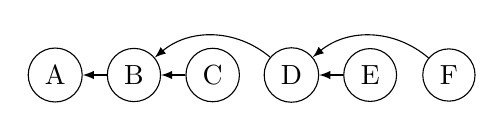
\begin{tikzpicture}[every node/.style={draw,circle},every edge/.style={draw,-latex}]
\node at (0.0, 0) (A) {A};
\node at (1, 0) (B) {B} edge (A);
\node at (2, 0) (C) {C} edge (B);
\node at (3, 0) (D) {D} edge[bend right=40] (B);
\node at (4, 0) (E) {E} edge (D);
\node at (5, 0) (F) {F} edge[bend right=40] (D);
\end{tikzpicture}
}
\item End to start: remove values inconsistent with parent
\item Start to end: assign any remaining consistent value
\end{enumerate}
\end{block}
}
\medskip
\visible<3->{Time complexity: \visible<4->{$O(nd^2)$}}
\end{frame}
\begin{frame}[label=tree-csp-example]{Tree-Structured CSP Example}
\begin{block}{Schedule jobs A, B, C, D, E for 9, 10, 11 or 12}
\begin{itemize}
\item B must be before 11:00
\item D must be after 10:00
\item B \& C must be after A
\item D \& E must be after C
\end{itemize}
\end{block}
\begin{center}
{\footnotesize
\begin{tikzpicture}[
  align=center,
  every node/.style={draw,circle,text width=4.1em,visible on={2-}},
  every edge/.style={draw,-latex,visible on={2-}}]
\node[filled on={11}] at (0.0, 0) (A) {{\normalsize A} \\ \scriptsize\{9\only<-9>{,10}\only<-7>{,11,12}\}};
\node[filled on={9,13}] at (2.3, 0) (B) {{\normalsize B} \\ \scriptsize\{\only<-9>{9,}10\}}
    edge (A);
\node[filled on={7,15}] at (4.6, 0) (C) {{\normalsize C} \\ \scriptsize\{\only<-7>{9,}10\only<-15>{,11}\only<-3>{,12}\}}
    edge[bend right=40] (A);
\node[filled on={5,17}] at (6.9, 0) (D) {{\normalsize D} \\ \scriptsize\{11\only<-17>{,12}\}}
    edge (C);
\node[filled on={3,19}] at (9.2, 0) (E) {{\normalsize E} \\ \scriptsize\{\only<-3>{9,}\only<-19>{10,}11\only<-19>{,12}\}}
    edge[bend right=40] (C);
\end{tikzpicture}
}
\visible<20>{}% trick Beamer into showing last frame
\end{center}
\end{frame}
\begin{frame}[label=decomposition]{Subproblems and Decomposition}
\begin{columns}[T]
\begin{column}{0.4\textwidth}
\begin{block}{Example}
Tasmania, mainland: separate components
\end{block}
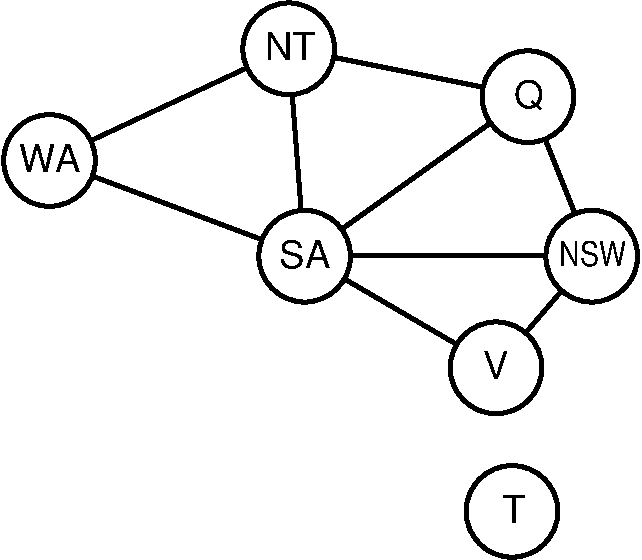
\includegraphics[width=\textwidth]{australia-csp.pdf}
\end{column}
\pause
\begin{column}{0.55\textwidth}
\begin{block}{If each subproblem has $c$ of the $n$ total variables}
\begin{itemize}
\item Num. of subproblems: \pause$n/c$
\pause\item Time per subproblem: \pause$d^c$
\pause\item Total work: \pause$O(nd^c/c)$
\end{itemize}
\end{block}
\pause
\begin{block}{$n=80, d=2, c=20$}
At 10 million nodes/sec:
\begin{itemize}
\item $2^{80} =$ 4 billion years 
\item $4 \cdot 2^{20} =$ 0.4 seconds
\end{itemize}
\end{block}
\end{column}
\end{columns}
\end{frame}
\begin{frame}[label=tree-decomposition]{Tree Decomposition}
	Convert constraint graphs to trees by assigning variables:
	\begin{center}
		\visible<2->{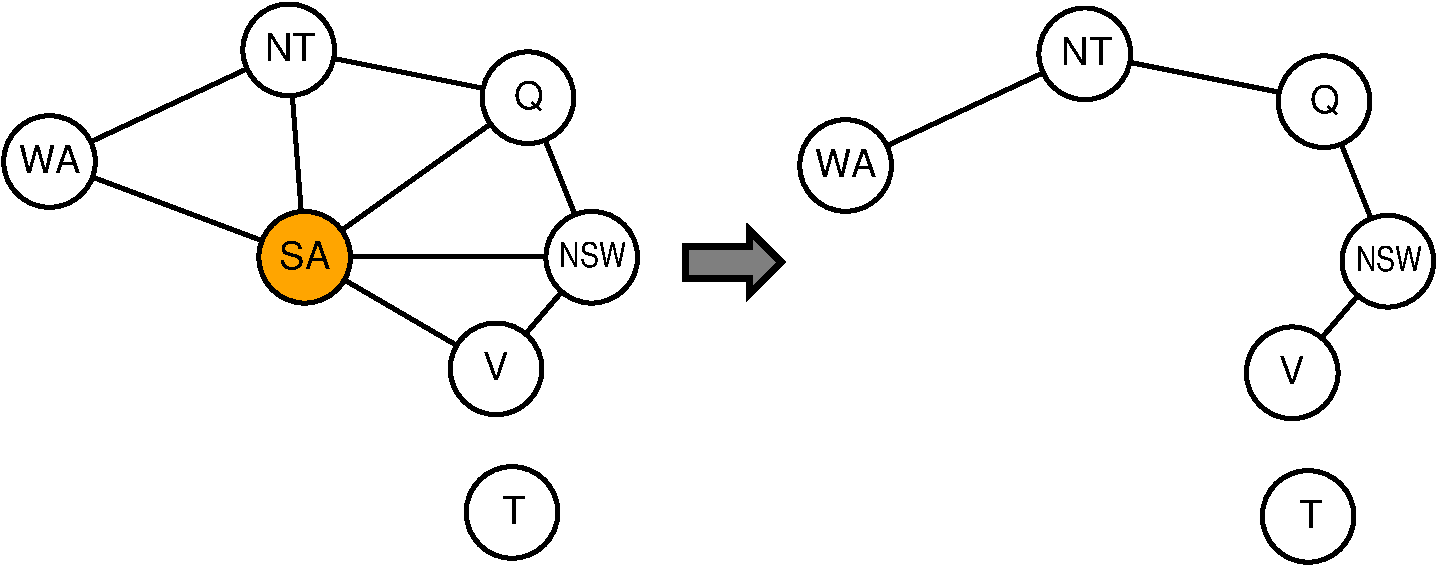
\includegraphics[width=3.5in]{australia-cutset.pdf}}
	\end{center}
	\begin{block}<3>{Properties}
		\begin{itemize}
			\item Complexity: \pause $O(d^c \cdot (n-c)d^2)$, given cutset size $c$
			\item Finding the smallest cycle cutset is NP-hard, but some efficient approximations exist
		\end{itemize}
	\end{block}
\end{frame}

\part{Key Points}
\begin{frame}{Key Points}
	\begin{block}{Constraint Satisfaction Problems}
		\begin{itemize}
			\item States are assignment of values to variables
			\item Goals are assignments with no constraint violations
		\end{itemize}
	\end{block}
	\begin{itemize}
		\item Backtracking \\			
			\begin{itemize}
				\item Depth-first search, one variable assigned per node
				\item Can be made effective with a number of heuristics
			\end{itemize}
		\item Min-Conflicts \\
			\begin{itemize}
				\item One value changed to reduce violations per iteration
				\item Usually effective in practice
			\end{itemize}
		\item Tree-Structured Search \\
			\begin{itemize}
				\item Can be solved in linear time
				\item Graphs can sometimes be decomposed into trees
			\end{itemize}
	\end{itemize}
\end{frame}

\end{document}


